\subsection{用户权限管理}
DBMS最有用的特性之一便是其完善健全的用户权限管理机制。考虑数据库的日常使用场景,为不同的用户(更正确的说,角色)提供不同级别、不同类型的权限是很有必要的。
\subsubsection{角色 (Roles)}
PostgreSQL为管理“用户”及其权限提供了\emph{角色}机制,在此机制下,“用户”、“用户组”是同一个概念,这点与MySQL等数据库的机制有十分关键的区别。
\par 
用户与用户组实际上都作为“角色”存储在\emph{pg\_roles}数据库中,自然,他们拥有同样数目的属性。使用DBMS的用户拥有一个\emph{登录角色 (login role)},同时,它可以从另一个角色继承权限,成为其 \emph{成员角色 (member role)},同时,拥有一些成员角色的角色现在被命名为 \emph{组角色 (group role)}。一般来说,出于安全性考虑,组角色不授予登录权限\textsuperscript{\cite{be-2017}},因为组角色被设计成一个权限集合,以便于管理多个用户的权限,而不是作为一个真正需要登录权限的用户的角色。从Postgres 8开始,我们可以用create user来明确指出创建的角色是一个普通的用户账户,其默认赋予可登录权限;而create role所创建的角色被Postgres认为可能作为组角色,默认是不具登陆权限 (cannot login) 的\textsuperscript{\cite{obe-2017}},这也是Postgres中“用户”与“用户组”最核心的区别。\\
\begin{figure*}[!h]
	\centering
	\begin{subfigure}[b]{0.8\textwidth}
		\centerline{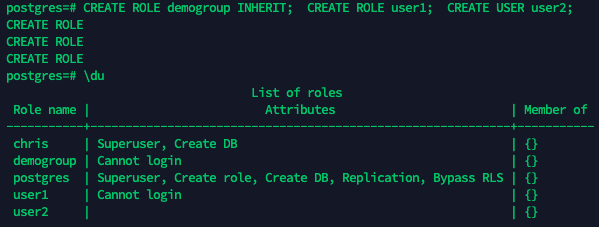
\includegraphics[height=2.5cm]{./pic/role1.png}\quad 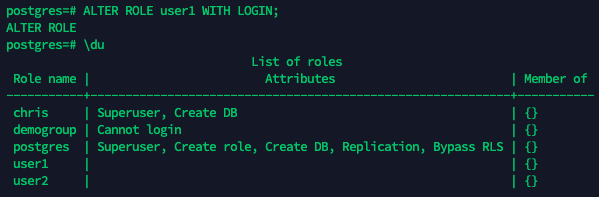
\includegraphics[height=2.5cm]{./pic/role2.png}}
		\caption{创建两个可登录角色、一个不可登录角色(组角色;\emph{INHERIT}关键词可省略)}
	\end{subfigure}
	\\~\\
	\begin{subfigure}[b]{0.8\textwidth}
		\centerline{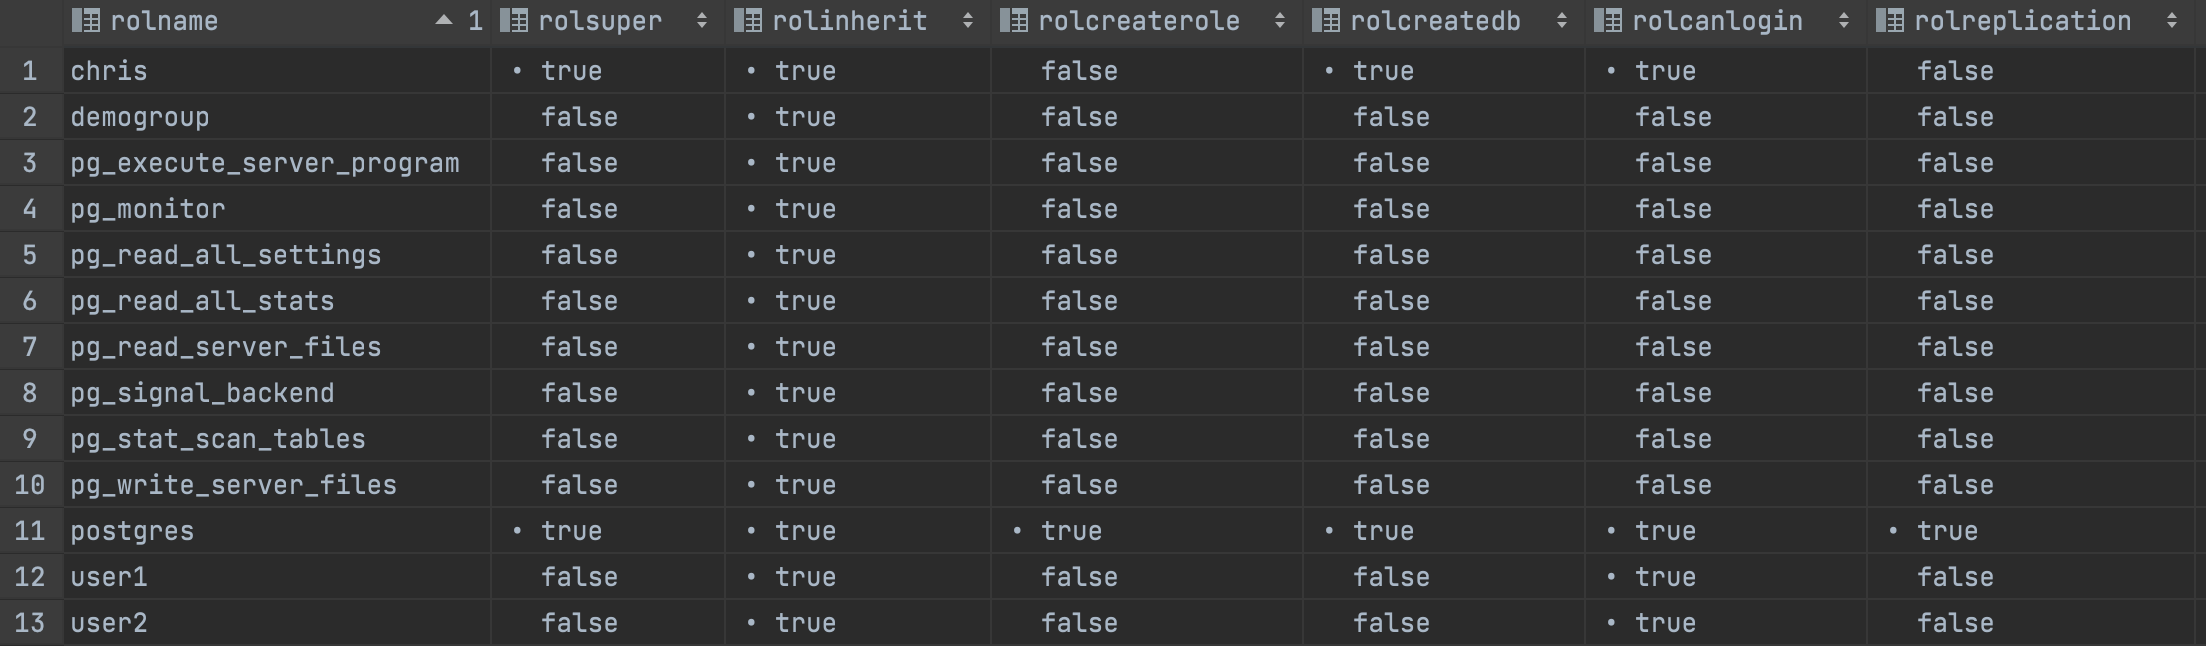
\includegraphics[width=\textwidth]{./pic/pgr.png}}
		\caption{SELECT * FROM  pg\_roles;}
	\end{subfigure}
	\\~\\
	\hspace{-2.3cm}
	\begin{subfigure}[b]{0.5\textwidth}
		\centerline{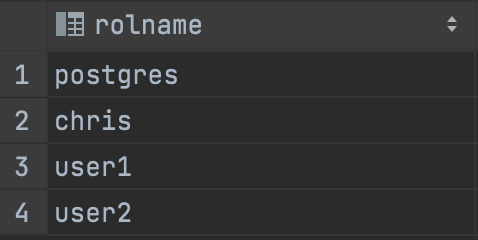
\includegraphics[height=2.5cm]{./pic/pgrw.png}}
		\caption{SELECT * FROM pg\_roles WHERE rolcanlogin;}
	\end{subfigure}
	\quad
	\begin{subfigure}[b]{0.3\textwidth}
		\vspace{-2.5cm}
		\centerline{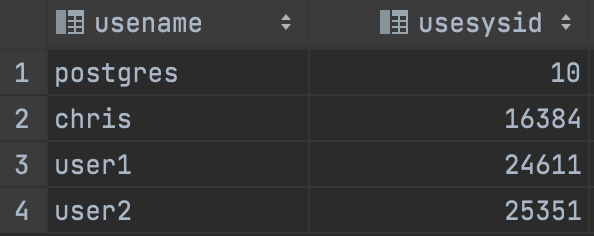
\includegraphics[height=2.5cm]{./pic/pgu.png}}
		\caption{SELECT * FROM  pg\_user;}
	\end{subfigure}
\end{figure*}

\indent 上图 (b) 和 (d) 
示PostgreSQL 13.3中依然有“用户”的概念,但其只是作为\emph{可登录角色}的别名\textsuperscript{\cite{psqldoc, unknown-author-2014}}。
\centerline{CREATE USER [usr] = CREATE ROLE [usr] WITH LOGIN}
\par
尽管Postgres中的“组角色”也可以作为另一个组角色的成员角色,这种嵌套关系是不限层数的,但一般为了安全性,DBA需要避免过多层组角色的继承以避免无意的为不该拥有某权限的角色授权。

% 越权与权限授予、收回
\subsubsection{权限授予}
当DBMS收到一条请求后,在首先检查其语法无误后,DBMS会检查发送请求的角色(\emph{role})及其是否有相应权限。如下图所示,如果发送SQL请求的角色没有对应权限,DBMS将拒绝该请求。为角色授权的语法如下\textsuperscript{\cite{unknown-author-2021}}:
\begin{lstlisting}
GRANT { { SELECT | INSERT | UPDATE | DELETE | TRUNCATE | REFERENCES | TRIGGER }
    [, ...] | ALL [ PRIVILEGES ] }
    ON { [ TABLE ] table_name [, ...]
         | ALL TABLES IN SCHEMA schema_name [, ...] }
    TO role_specification [, ...] [ WITH GRANT OPTION ]
\end{lstlisting}
\vspace{-2em}

\centerline{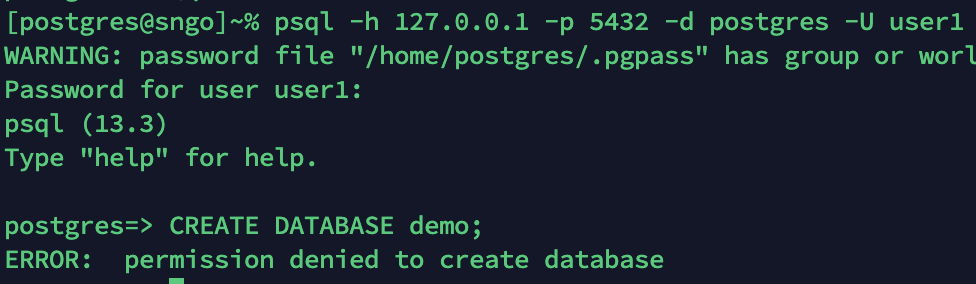
\includegraphics[width=0.65\textwidth]{./pic/nopriv.png}}
\vspace{1em}
\centerline{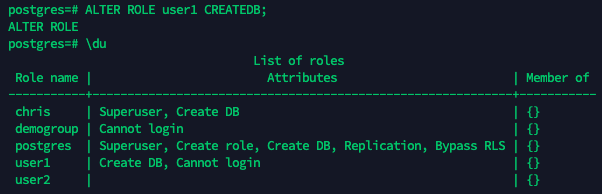
\includegraphics[height=2.5cm]{./pic/cdb.png}\quad 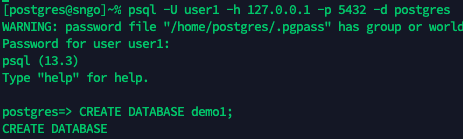
\includegraphics[height=2.5cm]{./pic/u1cdb.png}}

\par
特别地,一个“对象”(schema、table等)的所有者自然拥有该对象的所有权限。然而,作为对象的所有者并不意味着其是该对象的所有子对象的所有者(见下页图(c))。比如,如果一个角色创建并拥有一个数据库,而另一个角色在此数据库中创建了一个schema,则该对象默认并没有权限去访问此schema,但可以直接删除它。
\par
只有权限的拥有者(其必须同时拥有该权限的grant权限)可以将权限授予其他角色,而有些权限只能由对象的拥有者持有,如DROP和ALTER。另外,当授予一个角色时,可以通过添加WITH GRANT OPTION来允许该角色授予其他角色。
\par
当创建一个新的数据库时,DBMS会默认创建一个名为\emph{public}的schema,并将该schema的访问权授予一个名为public的角色。所有新的用户和角色都被默认授予public角色中的所有权限,因此所有人都可以在此public schema中创建对象。\\~\\
\centerline{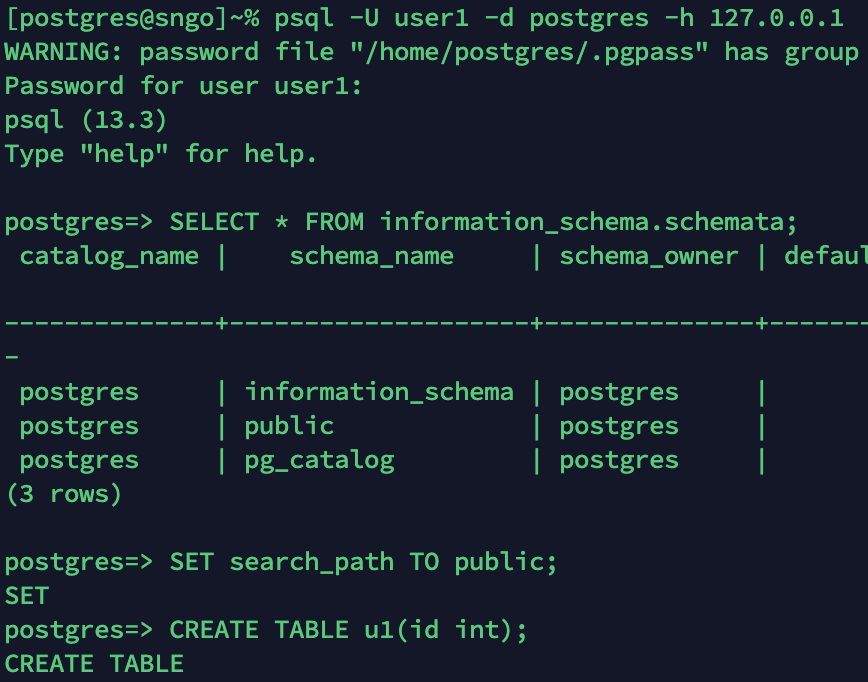
\includegraphics[width=0.6\textwidth]{./pic/mov.png}}
\begin{figure*}
	\centering
	\begin{subfigure}[b]{0.8\textwidth}
		\centerline{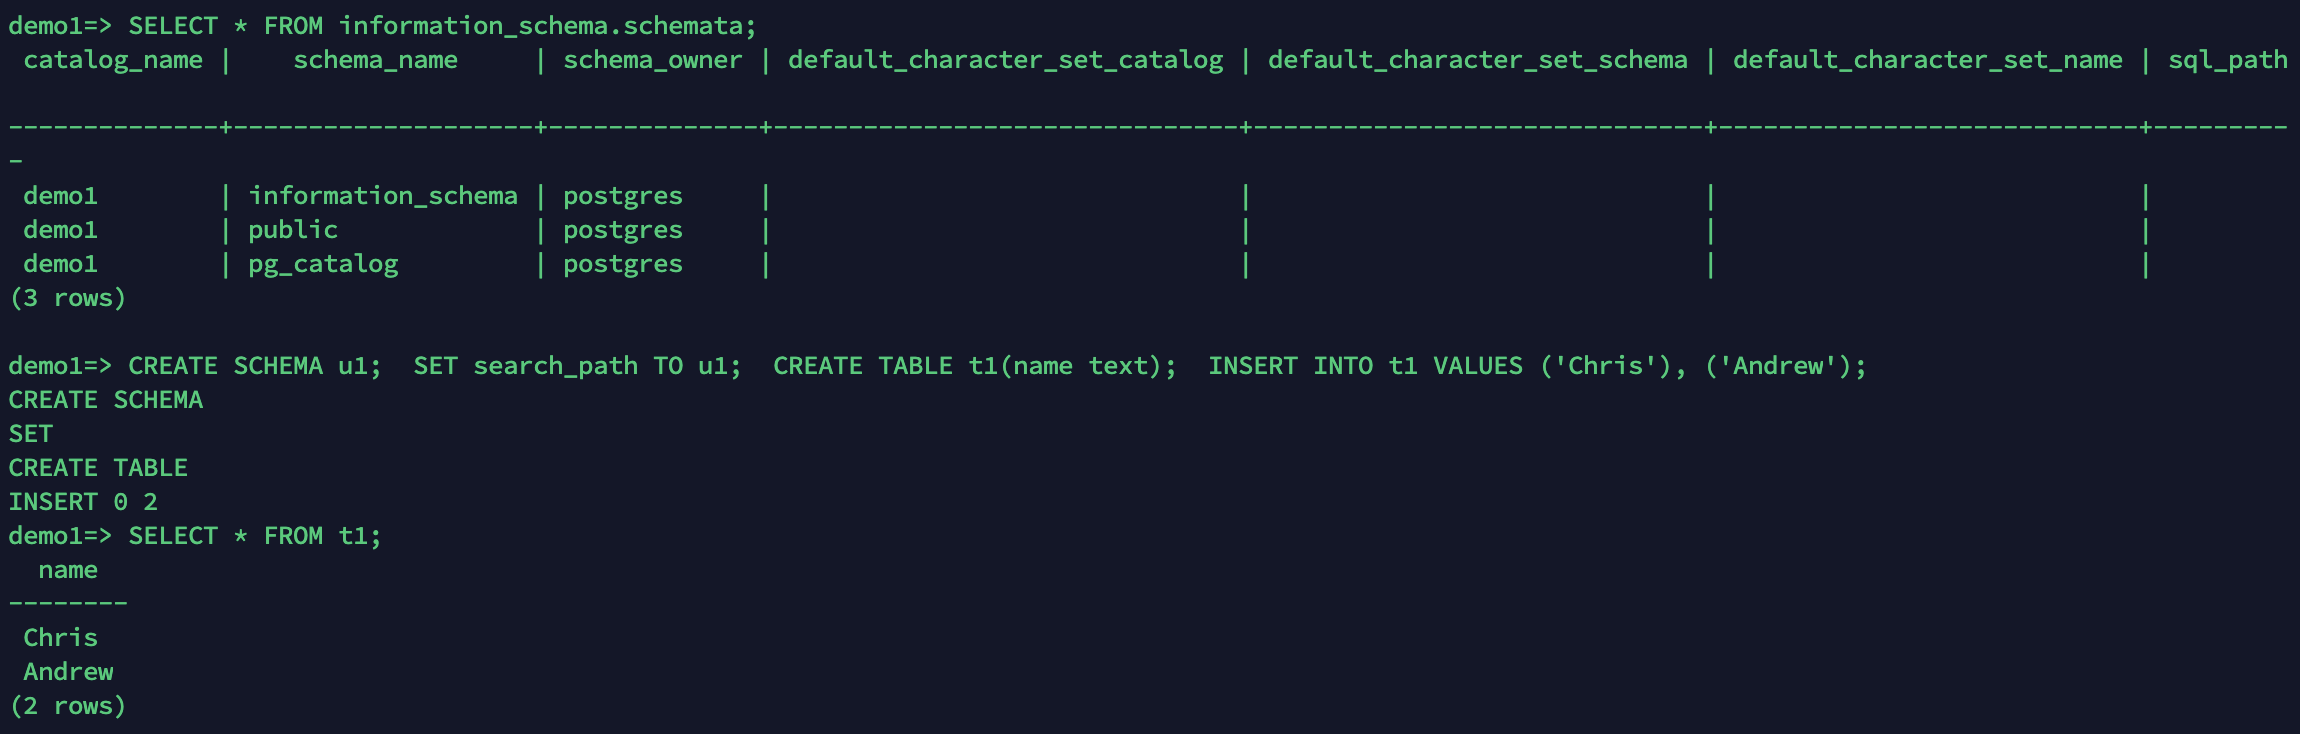
\includegraphics[height=3.6cm]{./pic/ins.png}}
		\caption{对象的创建者自动拥有该对象的所有权限}
	\end{subfigure}
	\\~\\
	\begin{subfigure}[b]{0.8\textwidth}
		\centerline{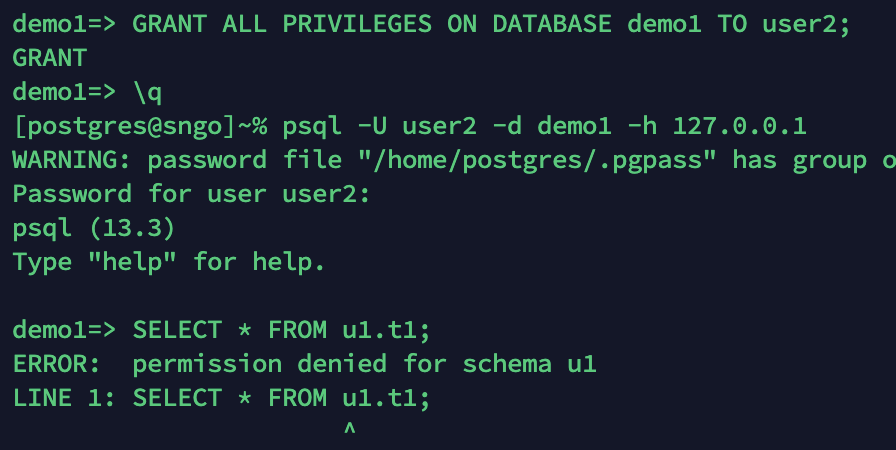
\includegraphics[width=0.6\textwidth]{./pic/grdb_nsch.png}}
		\centerline{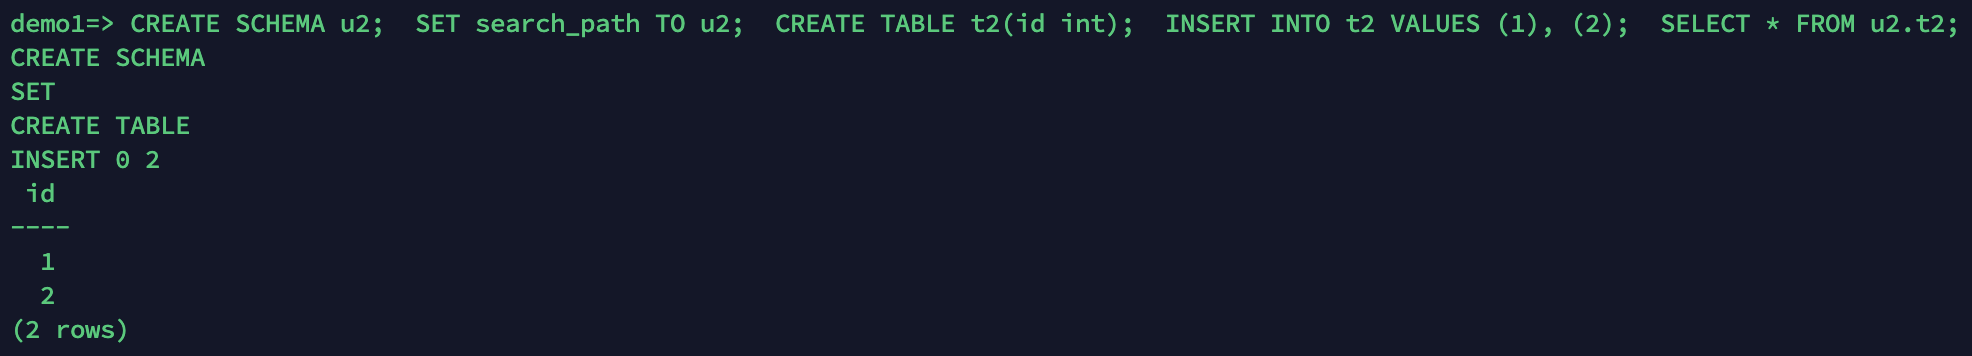
\includegraphics[width=0.6\textwidth]{./pic/u2.png}}
		\caption{角色被授予某数据库的所有权限后,依然不能访问特定的schema(除public外,由其他角色创建),但可以对数据库进行其他操作}
	\end{subfigure}
	\\~\\
	\begin{subfigure}[b]{0.8\textwidth}
		\centerline{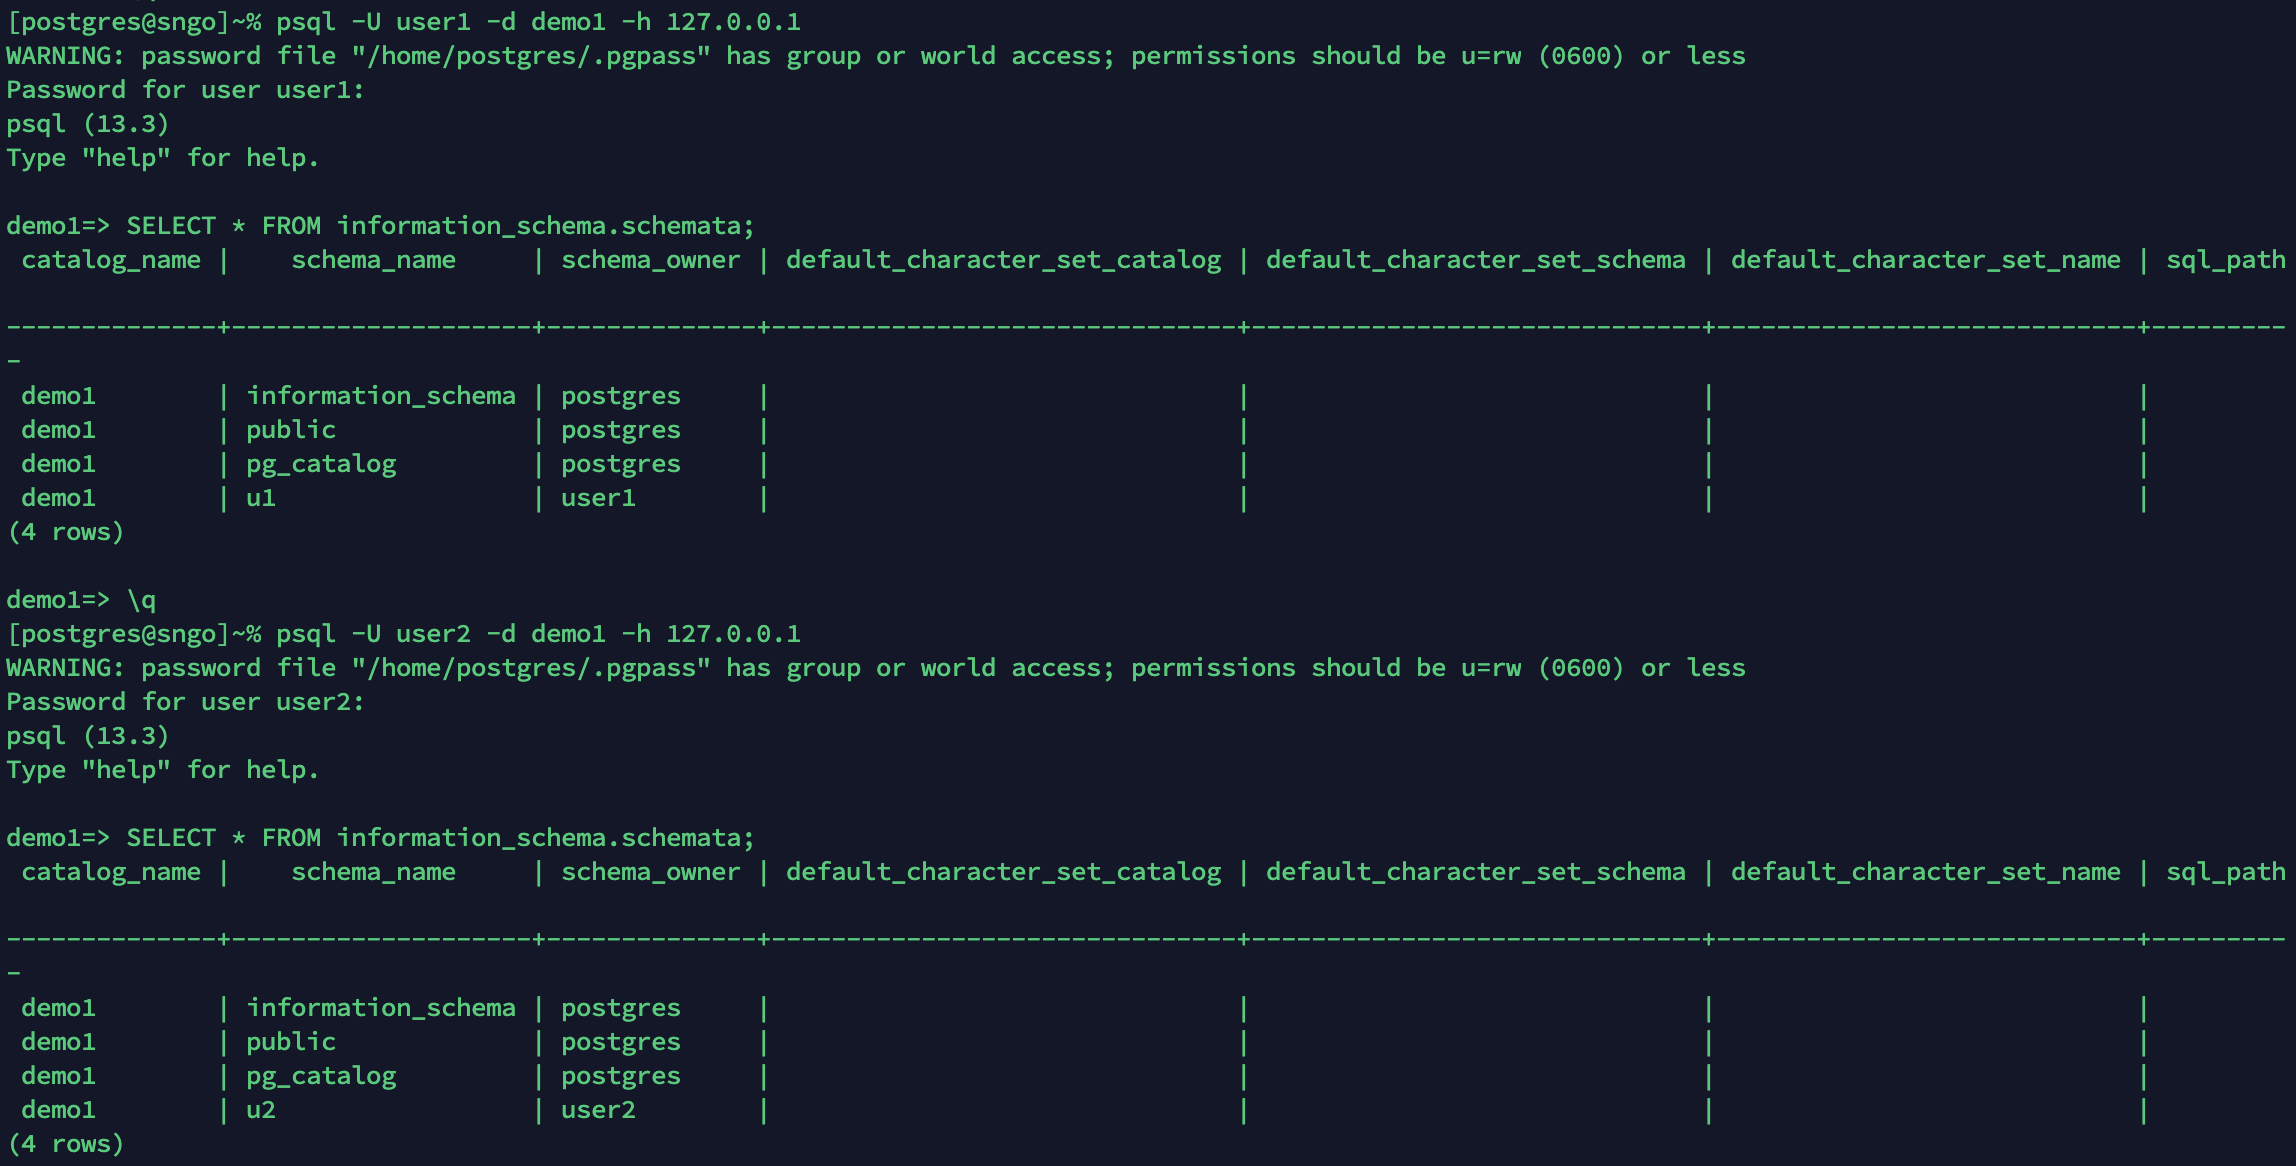
\includegraphics[width=\textwidth]{./pic/nvsb.png}}
		\caption{user2在user1所拥有对数据库中创建的schema对user1不可见}
	\end{subfigure}
	\\~\\
	\begin{subfigure}[b]{0.8\textwidth}
		\centerline{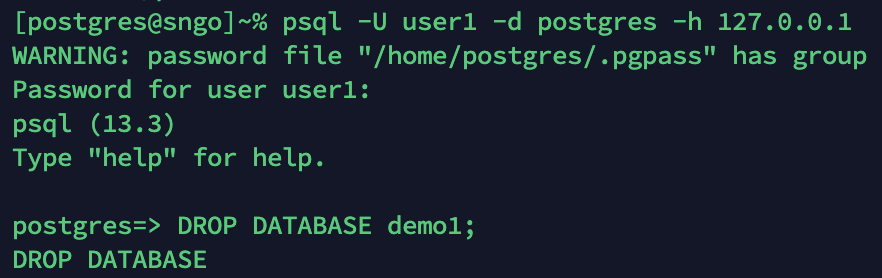
\includegraphics[width=0.6\textwidth]{./pic/ddpu1.png}}
		\caption{user1未被授予schema u2的相关权限,但因为其拥有整个数据库,因此可以直接将其drop}
	\end{subfigure}
	\label{fig:visual_smap}
\end{figure*}
\pagebreak


\subsubsection{撤回权限}
收回权限的语法与授权的语法类似:
\begin{lstlisting}
REVOKE [ GRANT OPTION FOR ]
    { { SELECT | INSERT | UPDATE | DELETE | TRUNCATE | REFERENCES | TRIGGER }
    [, ...] | ALL [ PRIVILEGES ] }
    ON { [ TABLE ] table_name [, ...]
         | ALL TABLES IN SCHEMA schema_name [, ...] }
    FROM role_specification [, ...]
    [ CASCADE | RESTRICT ]
\end{lstlisting}
\vspace{-2em}
\centerline{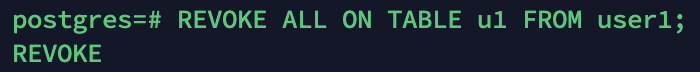
\includegraphics[width=0.5\textwidth]{pic/rvk}}
\par 在Postgres中较为特殊的一点是,删除角色时,一般不能直接删除,而要先将该角色被授予的所有权限收回,并转移其拥有的对象的所有权。\\~\\
\centerline{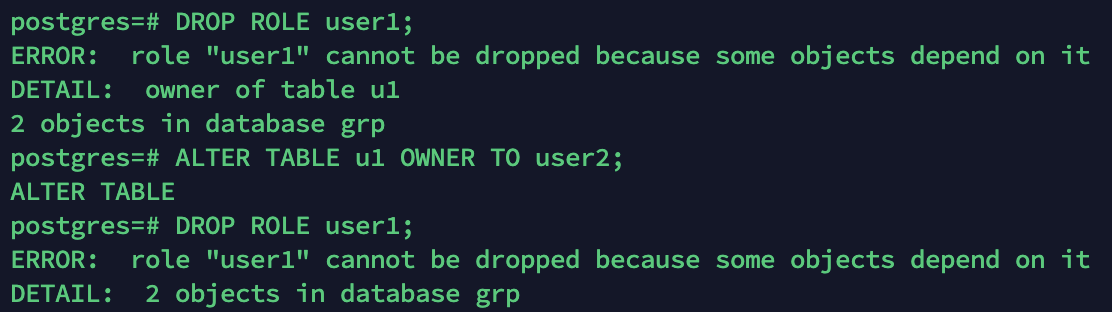
\includegraphics[width=0.7\textwidth]{pic/fail2dr}}

\subsubsection{组角色}
在前两小节的演示角色的图(a)中我们创建了一个名为\emph{demogroup}的组角色, 现用角色\textit{postgres}创建一个数据库,并将其所有权限赋予给该组角色。注意我们至始至终没有给user1授予权限。接下来,通过\\
\centerline{GRANT [group\_role] TO [login\_role];}
命令将user1和user2加入demogroup的成员角色。下图演示了进入组角色的user1自动继承了组中所有权限,我们得以在不直接对user1授权的情况下使user1有权操作该数据库。\\~\\
\centerline{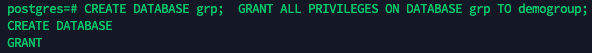
\includegraphics[width=0.7\textwidth]{./pic/grp.png}}
\centerline{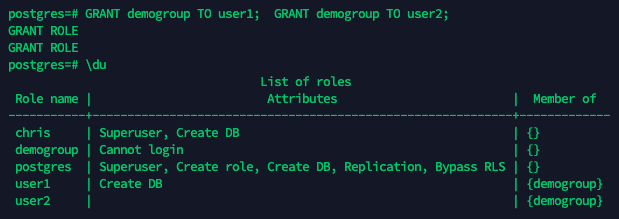
\includegraphics[width=0.7\textwidth]{./pic/grgrp.png}}
\centerline{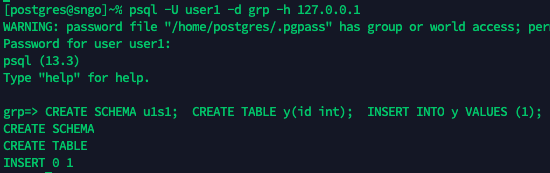
\includegraphics[width=0.7\textwidth]{./pic/grgrp2.png}}
\par 要删除一个组角色,执行DROP ROLE [group\_role]命令即可。在删除该组角色之后,它与其成员角色之间的关系将被立即撤销,而成员角色本身不受影响。需要注意的是,在删除前任何属于该组角色的对象都必须先被删除或者将对象的所有者转移给其它角色,与此同时,任何赋予该组角色的权限也都必须被撤消\textsuperscript{\cite{turing-2021}} 。
\subsubsection{文件系统用户权限管理}
文件系统可以通过改变文件的权限(以UNIX系OS为例,一般我们关注读、写、可执行权限)来达到类似的效果,通过系统自带的用户机制可以为不同用户、针对某个文件,分配不同的权限。\\~\\
\centerline{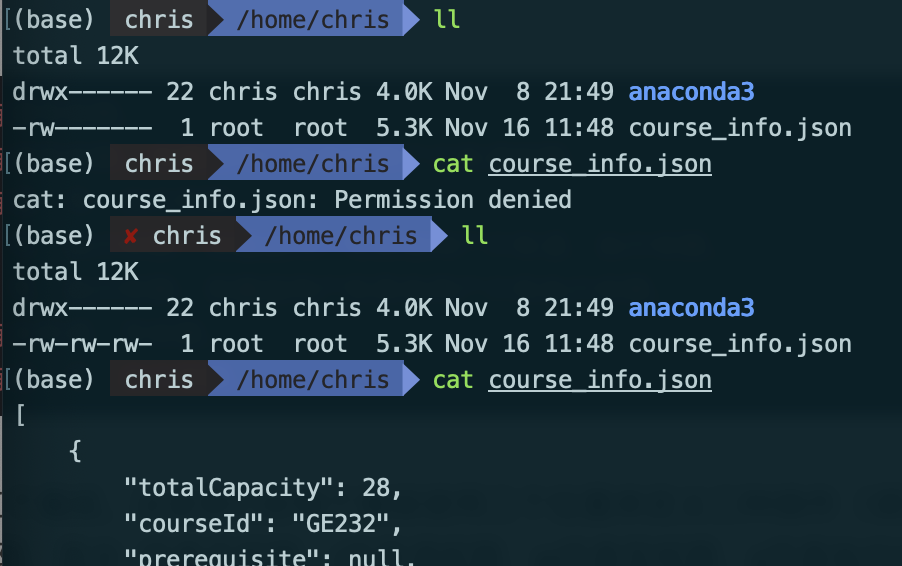
\includegraphics[width=0.55\textwidth]{pic/fsp}}
\par 上图演示在CentOS中使用root账号创建文件,并执行\textbf{chmod 600}命令使文件仅创建者可读写(如第一个ll所示),此时登录另一账号尝试读取文件,权限不足被拒;再次执行\textbf{chmod 666}对所有用户开放读写权限(如第二个ll所示),再次读取文件则成功显示内容。